\subsection{Упрощённое моделирование треков частиц}

Ряд техник сопоставления с
образцом~(англ.~\emph{pattern matching}, \cite{MankelTracking}) при
предварительном трекинге требуют
идеализированной информации о движении частицы. Для этого, а так же с тем чтобы
оценить вклад отдельных факторов в ошибки реконструкции треков
частиц удобно использовать численное моделирование (например, методы
Монте-Карло). В то же время, методы Рунге-Кутты применяемые для обобщённого
описания движения частицы в магнитном поле, используются и при реконструкции
трека и методически неверно использовать их и для моделирования.

Чтобы построить простейшую модель трекера NA64, ограничимся следующими
допущениями:
\begin{itemize}
    \item Рассмотрим движение в однородном постоянном магнитном поле, заданном
    в прямоугольном объёме;
    \item Потери энергии частицы (на ионизацию и излучения), а
    также изменение направление движения вследствие рассеяния на веществе
    детекторов не учитываются;
    \item Чувствительную область описывается двумя векторами --
    единичным вектором измерения координаты $\vec{u}$ и вектором направления
    чувствительных элементов $\vec{v}$ (проволок, литографических полос,
    разрядных трубок и т.д.).
\end{itemize}
Таким образом, моделирование частицы сведётся к простейшей задаче тассировки
индивидуальных частиц функциями-пропагаторами двух типов: луча и винтовой
линии до пересечения с плоскостями ограниченными параллелограммом постренным
на векторах $\vec{u}$ и $\vec{v}$. Прямоугольный объём заключающий магнитное
поле можно описать в тех же терминах, что и чувствительную область детектора.

\subsubsection{Прямолинейное движение}

Пересечение прямолинейной траектории заданной параметрическим
уравнением~$\vec{r}(s) = \vec{r}_{t,0} + \vec{p} \cdot s$ с плоскостью
проходящей через точку~$\vec{r}_{p,0}$ разрешается простой подстановкой:
\begin{equation}
    s = \frac{\vec{n}(\vec{r}_{t,0} - \vec{r}_{p,0})}{\vec{n} \vec{p}}.
    \label{eq:trackletPlaneIP}
\end{equation}

Размерность параметра $s$ удобно выбрать таким образом чтобы он соответствовал
времени движения частицы.

\subsubsection{Движение в постоянном магнитном поле}

Винтовую линию зададим следующим образом \cite{StrandlieJacobians}:
\begin{equation}
    \vec{r} = \vec{r}_0 + \frac{\delta}{K} (\theta - \sin \theta ) \cdot \vec{h} + \frac{\sin \theta}{K} \cdot \vec{t}_0 + \frac{\alpha}{K} (1 - cos \theta) \cdot \vec{n}_0,
    \label{eq:helixMovement}
\end{equation}
где:
\begin{description}
    \item $\vec{h} = \vec{B}/|B|$ единичный вектор индукции магнитного поля,
    \item $\vec{t} = \vec{p}/|p|$ единичный касательный вектор начального 
    направления движения частицы,
    \item $\vec{n} = (\vec{h} \times \vec{t})/\alpha$ вектор бинормали с
    единичным вектором $\alpha = |\vec{h} \times \vec{t}|$,
    \item $\delta = \vec{h} \cdot \vec{t}$,
    \item $K = -k \psi |\vec{B}|$ период вращательного движения ($k$ ---
    размерный коэффициент),
    \item $\psi = q/p$,
    \item $\theta = K s$ --- угловая фаза движения частицы.
\end{description}

\begin{figure}
     \centering
     \begin{subfigure}[b]{0.3\textwidth}
         \centering
         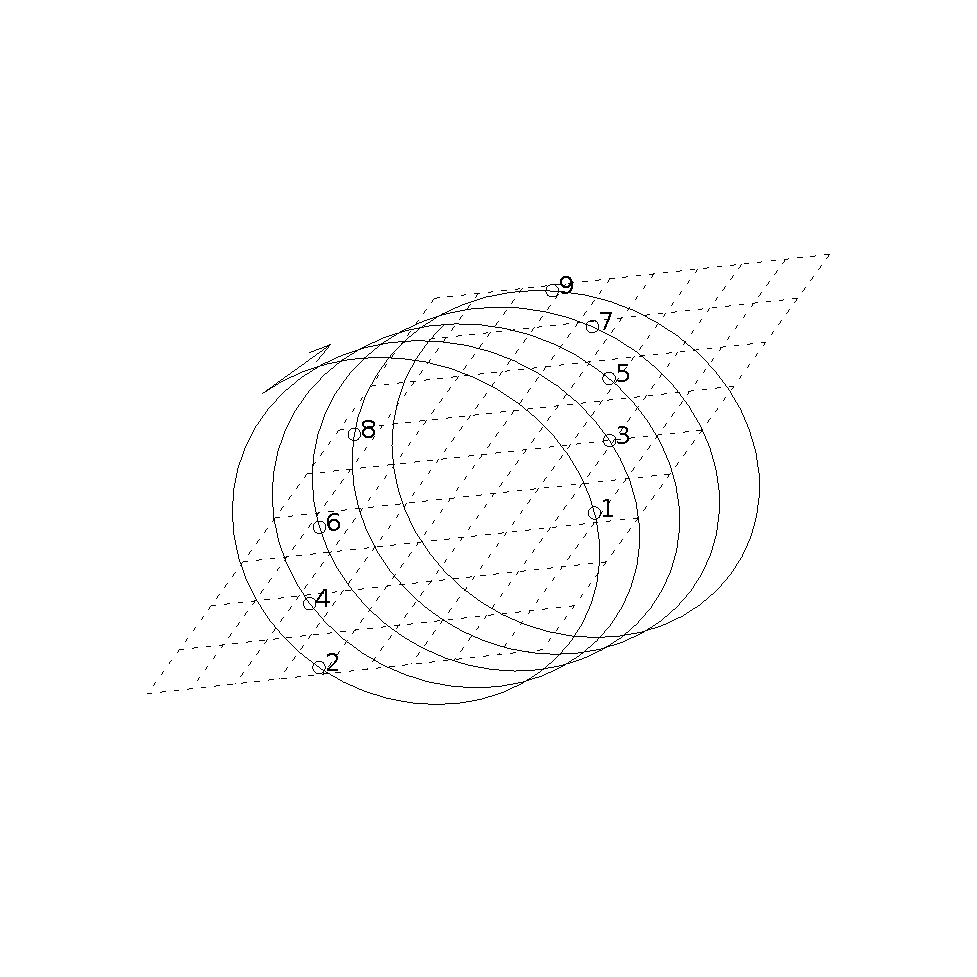
\includegraphics[trim={2.2cm 4cm 2cm 4cm},clip,width=.5,width=\textwidth]{images/arttrack/helix.eps}
         \caption{Винтовая линия, плоскость и точки пересечения в порядке
         заданном параметром $t$.}
         \label{fig:helixPlaneProblem}
     \end{subfigure}
     \hfill
     \begin{subfigure}[b]{0.6\textwidth}
         \centering
         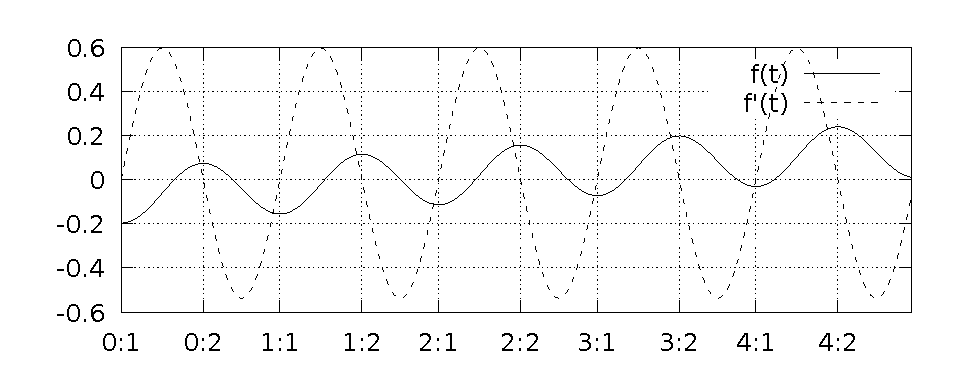
\includegraphics[width=\textwidth]{images/arttrack/helix-plane-func.eps}
         \caption{График функции проекции винтовой линии на нормаль плоскости.
         Отметки на горизонтальной оси соответствуют номеру периода и номеру
         экстремума в периоде.}
         \label{fig:hlxPlaneFuncAndDeriv}
     \end{subfigure}
        \caption{Изображение винтовой линии пересекающей плоскость и точек
            пересечения найденных при помощи численного метода в участках
            заданных \eqref{eq:helixPlaneExtrema}.}
        \label{fig:helixPlaneProblem}
\end{figure}

Для траектории заданной винтовой линией потребуется привлекать
численные методы, поскольку подстановка пропагатора \eqref{eq:helixMovement}
в уравнение плоскости приводит к трансцендентному уравнению с
произвольным числом корней
вида~$A \cdot \sin \theta + B \cdot \cos \theta + C \cdot \theta + D = 0$.
Участки монотонности этого трансцендентного уравнения заются двумя экстремумами
функции~\eqref{eq:helixMovement}:
\begin{equation}
    \theta_{1,2} = \pm \arcsin \frac{C}{\sqrt{A^2 + B^2}} - \arctan{\frac{B}{A}},
    \label{eq:helixPlaneExtrema}
\end{equation}
где $A = (\delta \vec{h} + \vec{t}_0) \cdot \vec{n}_p$,
$B = \alpha \vec{n}_p \cdot \vec{n}_0$, $C = \delta \vec{h} \cdot \vec{n}_p$.

Полностью, алгоритм отыскания пересечения винтовой линии
заданной~\eqref{eq:helixMovement} и плоскости выглядит следующим образом:
\begin{enumerate}
    \item Для заданного магнитного поля $\vec{B}$ импульса~$\vec{p}$ и
    заряда~$q$ частицы, отыскать экстремальные точки проекции касательного
    вектора на нормаль заданной плоскости~$\vec{n}_p$
    согласно~\eqref{eq:helixPlaneExtrema}, где $s > s_0$.
    \item Если корни \eqref{eq:helixPlaneExtrema} не определены (случай
    ориентации плоскости перпендикулярно полю), отыскание пересечения можно
    произвести численным методон последовательных приближений (напр. методом
    Ньютона), начиная с $s_0$.
    \item Подстановкой~\eqref{eq:helixPlaneExtrema} в~\eqref{eq:helixMovement}
    определить участки перемены знака и использовать в них численный метод
    отыскания нуля на отрезке (напр. дихотомий). При этом, если подстановка
    корней не приводит к уменьшению абсолютной величины среднего значения
    функции в течении двух последовательных периодов, считать, что пересечений
    с плоскостью нет (частица удаляется от плоскости).
\end{enumerate}
Реализация такого алгоритма должна предусматривать случай когда ось винтовой
линии
\begin{equation}
    \vec{l}(s) = \vec{r}_0 + \delta \vec{h} s + n_0 \alpha / K.
    \label{eq:helixAxis}
\end{equation}
параллельна плоскости --- то есть число корней~\eqref{eq:helixPlaneExtrema}
бесконечно.

Результат работы такого алгоритма представлен на рисунке~\ref{fig:helixPlaneProblem}.

\subsubsection{Определение локальных координат}

\begin{center}
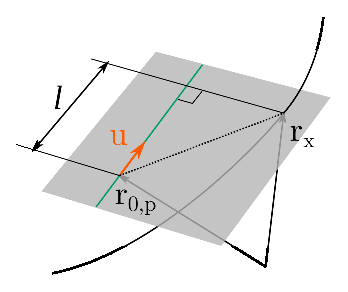
\includegraphics[width=.5\textwidth]{images/arttrack/arttrack-u-measurement.eps}
\end{center}

\subsubsection{Реализация}

\begin{figure}[ht]
    \centering
    \subfloat[Фронтальный вид]{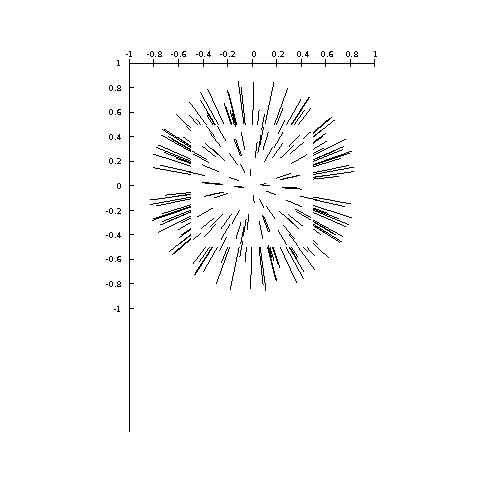
\includegraphics[trim={0 3cm 0 0},clip,width=.5\textwidth]{images/arttrack/box-in-sphere-ortho.eps}}
    % ^^^ trim={0 3cm 0 0},clip,
    \subfloat[Ортографическая проекция]{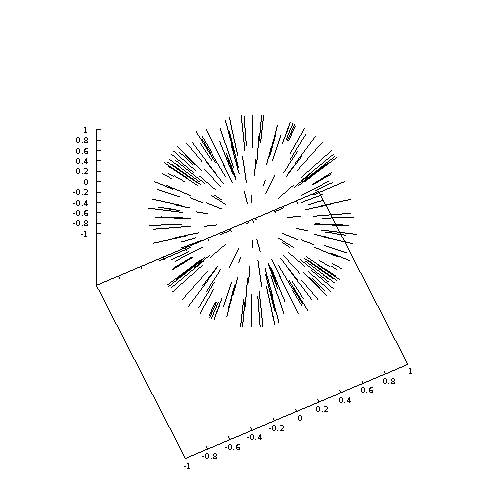
\includegraphics[width=.33\textwidth]{images/arttrack/box-in-sphere.eps}}
    \caption{Визуализации различных тестов.}
    \label{fig:boxInSphere}
\end{figure}